%%%%%%%%%%%%%%%%%%%%%%%%%%%%%%%%%%%%%%%%%%%%%%%%%%%%%%%%%%%%%%%%%%%%%%
% LaTeX Example: Project Report
%
% Source: http://www.howtotex.com
%
% Feel free to distribute this example, but please keep the referral
% to howtotex.com
% Date: March 2011 
% 
%%%%%%%%%%%%%%%%%%%%%%%%%%%%%%%%%%%%%%%%%%%%%%%%%%%%%%%%%%%%%%%%%%%%%%
% How to use writeLaTeX: 
%
% You edit the source code here on the left, and the preview on the
% right shows you the result within a few seconds.
%
% Bookmark this page and share the URL with your co-authors. They can
% edit at the same time!
%
% You can upload figures, bibliographies, custom classes and
% styles using the files menu.
%
% If you're new to LaTeX, the wikibook is a great place to start:
% http://en.wikibooks.org/wiki/LaTeX
%
%%%%%%%%%%%%%%%%%%%%%%%%%%%%%%%%%%%%%%%%%%%%%%%%%%%%%%%%%%%%%%%%%%%%%%
% Edit the title below to update the display in My Documents
%\title{Project Report}
%
%%% Preamble
\documentclass[paper=a4, fontsize=11pt]{scrartcl}
\usepackage[T1]{fontenc}
\usepackage{fourier}
\usepackage{apacite}
\usepackage[english]{babel}															% English language/hyphenation
\usepackage[protrusion=true,expansion=true]{microtype}	
\usepackage{amsmath,amsfonts,amsthm} % Math packages
\usepackage[pdftex]{graphicx}	
\usepackage{url}
\usepackage{hyperref}
\graphicspath{ {./PhyReportImg/} }

%%% Custom sectioning
\usepackage{sectsty}
\allsectionsfont{\centering \normalfont\scshape}


%%% Custom headers/footers (fancyhdr package)
\usepackage{fancyhdr}
\pagestyle{fancyplain}
\fancyhead{}											% No page header
\fancyfoot[L]{}											% Empty 
\fancyfoot[C]{}											% Empty
\fancyfoot[R]{\thepage}									% Pagenumbering
\renewcommand{\headrulewidth}{0pt}			% Remove header underlines
\renewcommand{\footrulewidth}{0pt}				% Remove footer underlines
\setlength{\headheight}{13.6pt}


%%% Equation and float numbering
\numberwithin{equation}{section}		% Equationnumbering: section.eq#
\numberwithin{figure}{section}			% Figurenumbering: section.fig#
\numberwithin{table}{section}				% Tablenumbering: section.tab#


%%% Maketitle metadata
\newcommand{\horrule}[1]{\rule{\linewidth}{#1}} 	% Horizontal rule

\title{
		%\vspace{-1in} 	
		\usefont{OT1}{bch}{b}{n}
		\normalfont \normalsize \textsc{Mr. Daoud | SPH3U1-ISP} \\ [25pt]
		\horrule{0.5pt} \\[0.4cm]
		\huge Physics ISP: Designing and Building a Bridge \\
		\horrule{2pt} \\[0.5cm]
}
\author{
		\normalfont 								\normalsize
        Robert Li, Josh Liu, and Mitchell Green\\[-3pt]		\normalsize
        \today
}
\date{}


%%% Begin document
\begin{document}
\maketitle
% \newpage
\tableofcontents{}
% \newpage
\section{Basic Research}
The triangle is considered the best shape for trusses because in many cases it is considered the strongest simple shape. If the three sides are made of rigid materials and pressure were to be applied top the shape, the joints of the shape have a better change of breaking than the shape does collapsing. Unlike a square that can effortlessly be pushed into a parallelogram or a hexagon which is easily deformed; unless it has triangular dividers inside. The triangle’s joints are fixed. It is fundamentally rigid in its design. The angels of an equilateral triangle cannot change.
\begin{center}
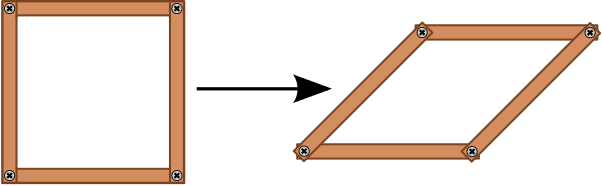
\includegraphics{square}
\end{center}
\subsection{Pratt Truss}
\begin{center}
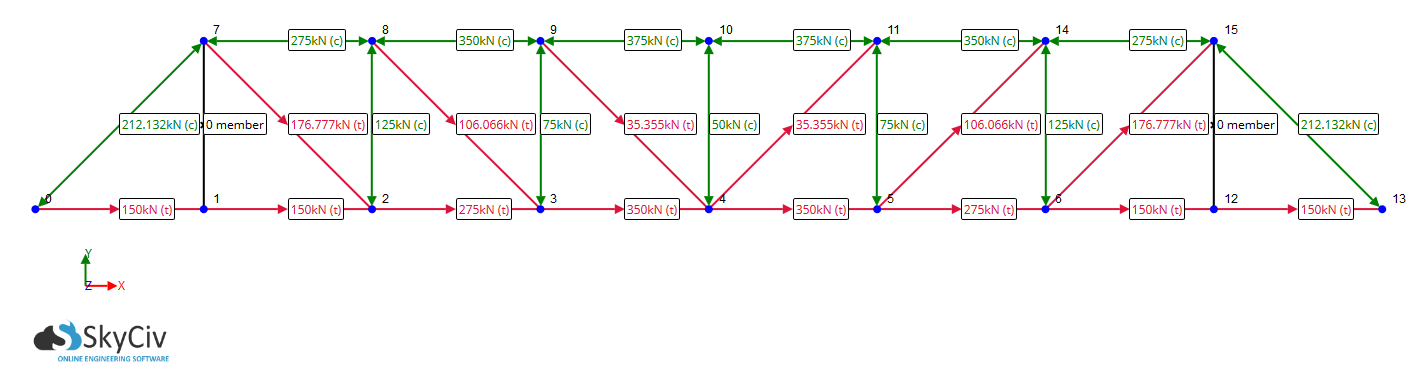
\includegraphics[scale=0.35]{PrattTruss}    
\end{center}

The Pratt truss bridge is one of the simplest designs of bridges. The supports on the bottom of the bridge as well as the diagonal supports are under tension. The supports in the vertical direction and on the top, however, are under compression. Its advantages are that this bridge usually fairs well under circumstances that have a concentrated weigh, it is usually is lightweight compared to some other models and it is simplistic. However, for our purposes, it has one fatal error. We are using wood for our building material and wood does not perform well under tension, which this bridge uses a lot of. Therefore, it would not be the logical choice.

\subsection{Howe Truss}

\begin{center}
    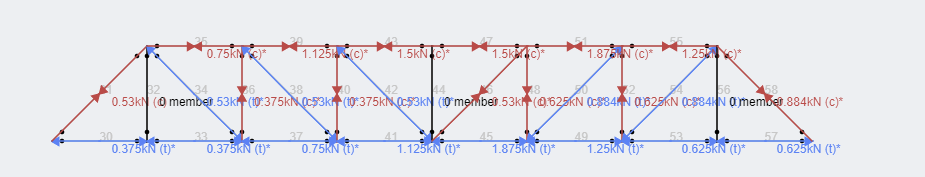
\includegraphics[scale=0.5]{HoweTruss}
\end{center}
A Howe Truss is very much like a Pratt Truss. It too is simple in design. The one major difference is that the slants on the diagonal supports are in the opposite direction. The supports in the vertical direction as well as the bottom supports are under compression. The supports on the top of the bridge as well as the diagonal supports, are under tension. This bridge also does well under concentrated weight tests, it is also lightweight, much like the Pratt truss, and it is also lightweight. However, it too has one fatal error. Because we are using wood as the medium for construction, the bridge would put too much tension force on the wood, causing it to potentially break. Much like its cousin, the pratt truss, this bridge would also not be the logical choice.

\subsection{Warren Truss}
\begin{center}
    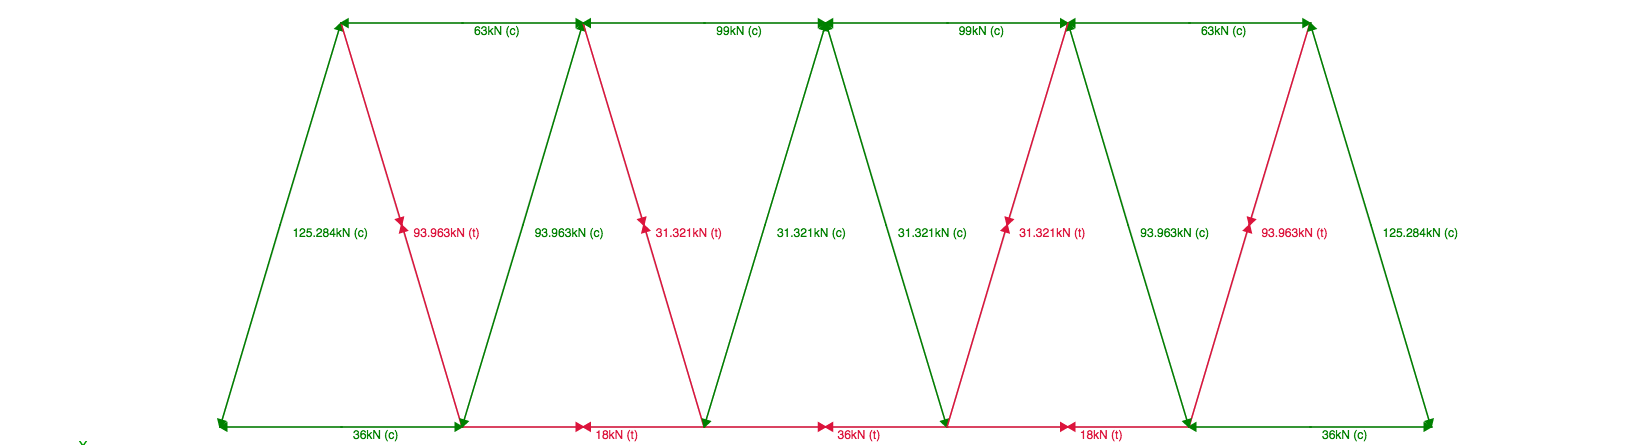
\includegraphics[width=0.5\textwidth]{WarrenTruss}
\end{center}
In the warren truss bridge, less than half of the slanted supports are under tension. Less than half of the bottom supports are under tension. None of the top supports are under tension. The first advantage of a warren bridge is that the design works to the advantage of the popsicle stick. Because less that 50\% is under tension, the compression strengthens our design. The truss is a fairly simple design that utilized the strength of equilateral triangles to its advantage. The inherent genius of its design is that it is a master of distributing forces

\section{Model of the bridge}
\begin{figure}[h!]
    \begin{center}
        \begin{minipage}{0.2\textwidth}
            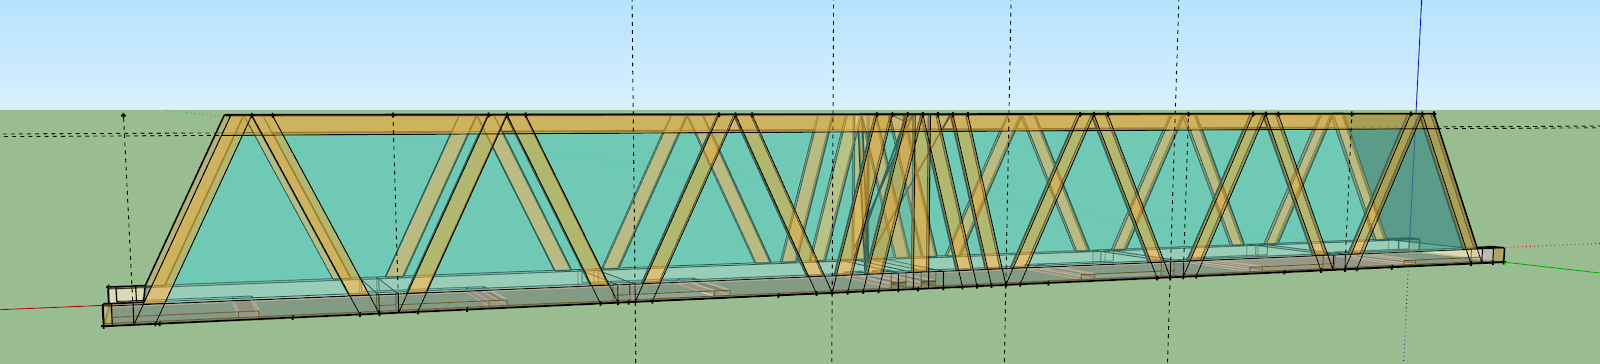
\includegraphics[width=\textwidth]{Model1}
        \end{minipage}
        \begin{minipage}{0.2\textwidth}
            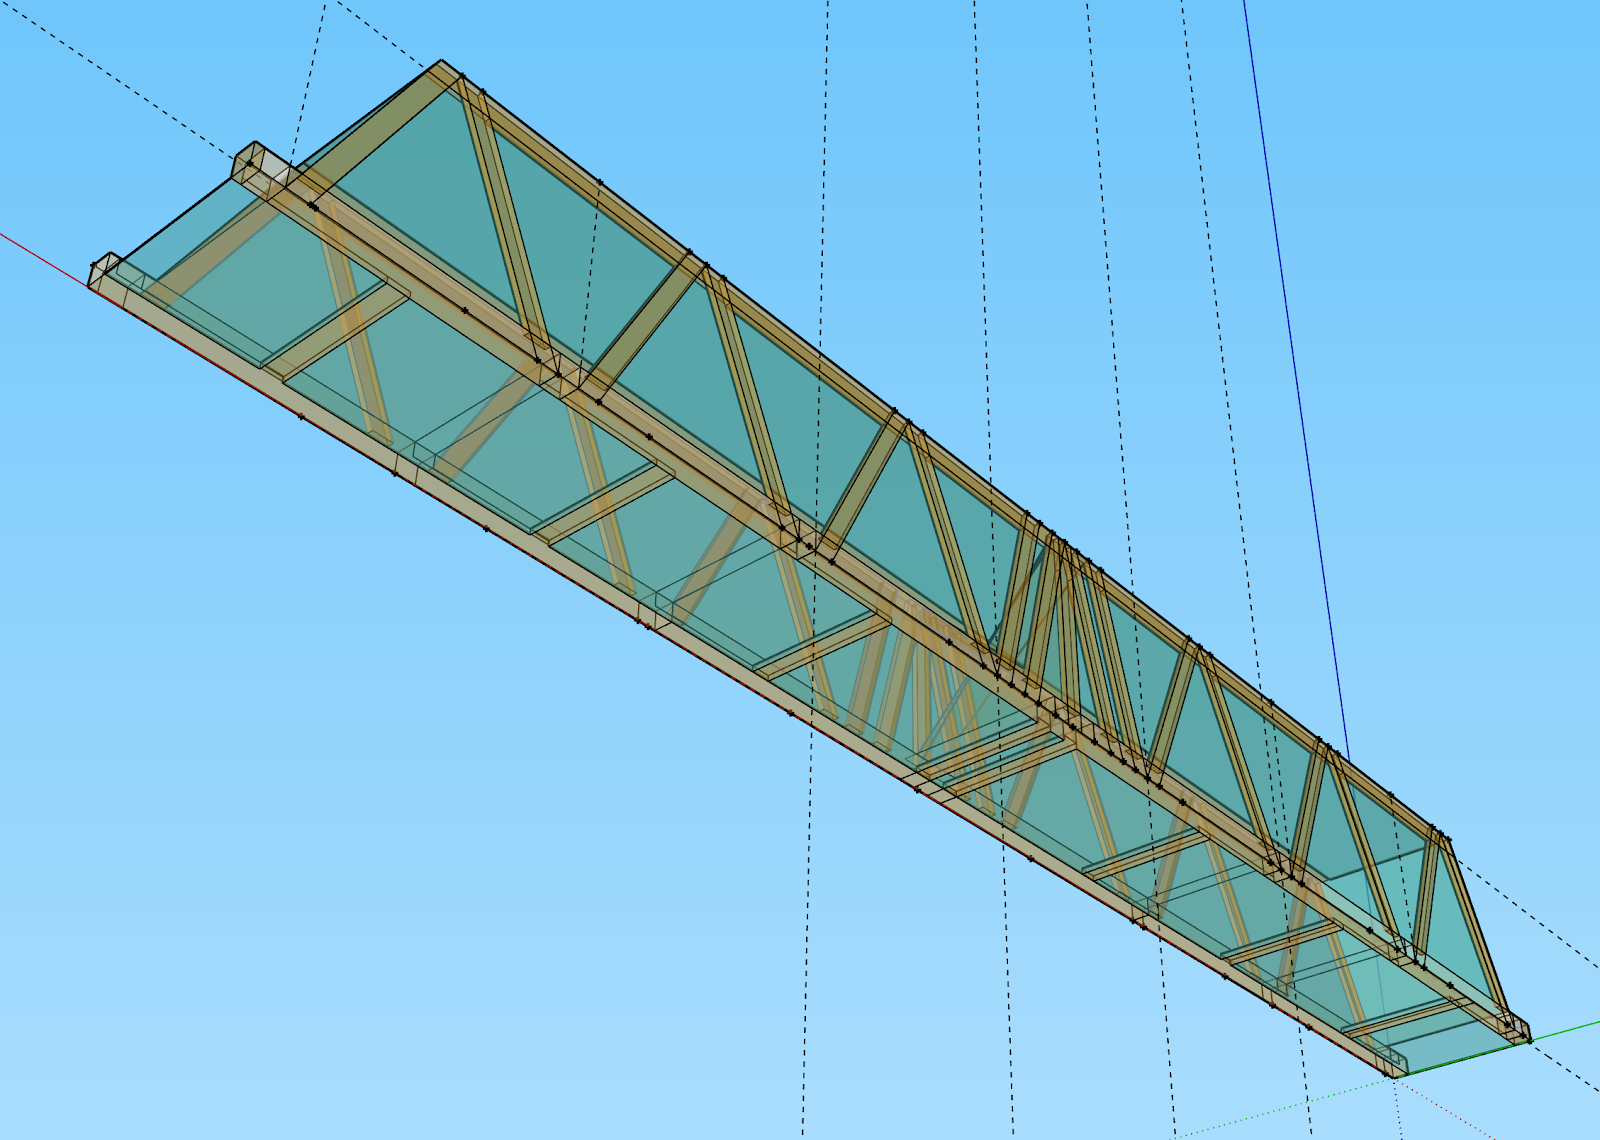
\includegraphics[width=\textwidth]{Model2}
        \end{minipage}
        \begin{minipage}{0.2\textwidth}
            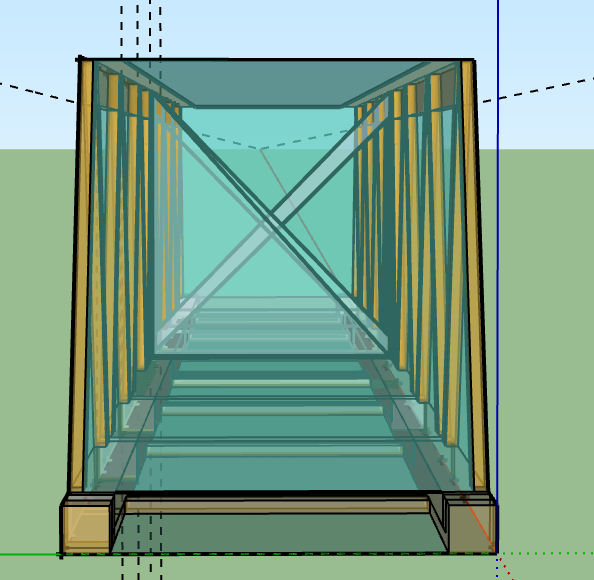
\includegraphics[width=\textwidth]{Model3}
        \end{minipage}
        \begin{minipage}{0.2\textwidth}
            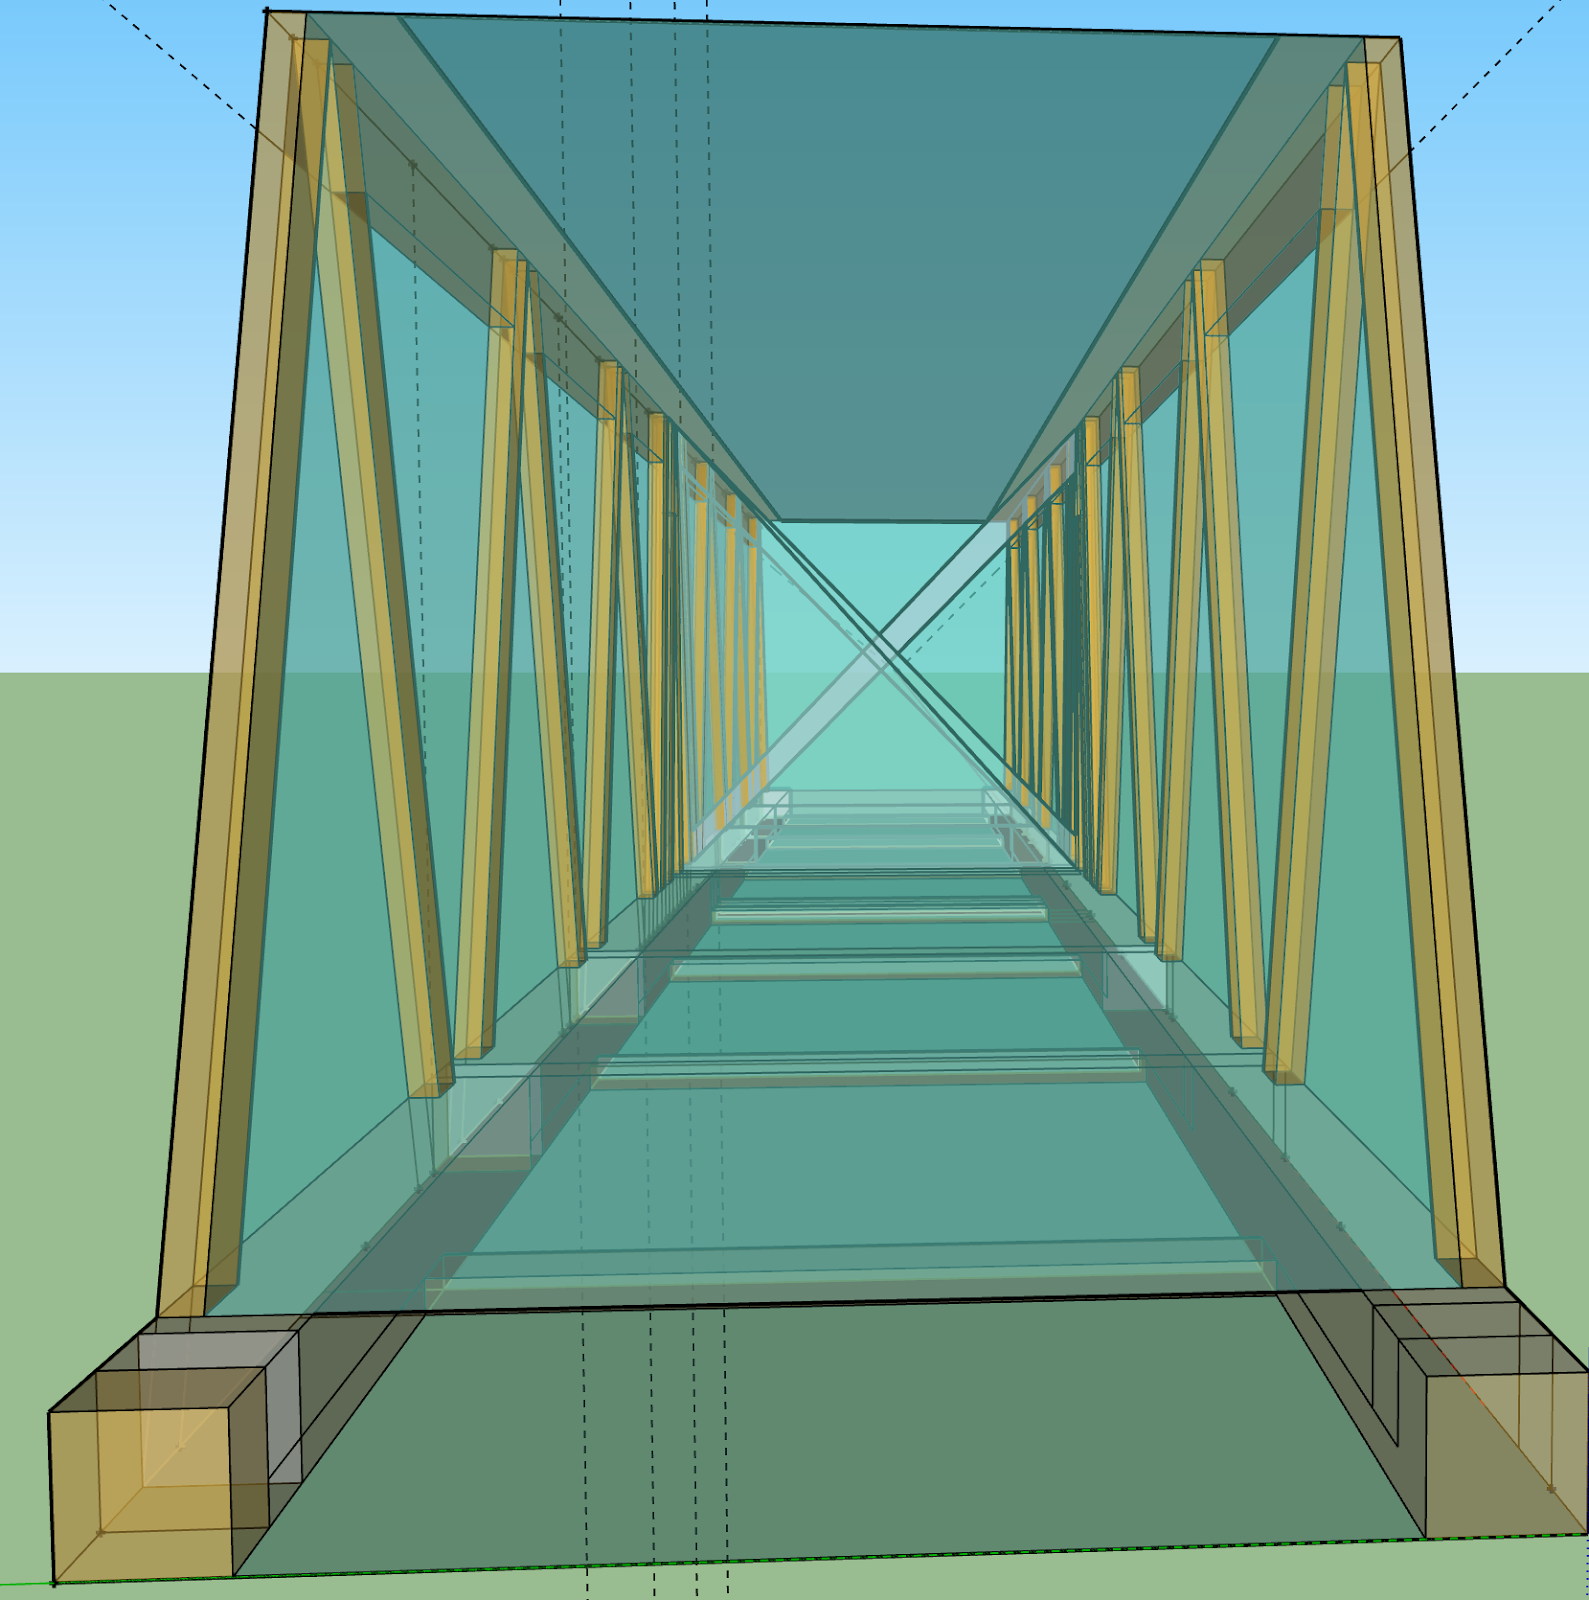
\includegraphics[width=\textwidth]{Model4}
        \end{minipage}
        \small A full 3D model can be seen \href{https://edu.sketchup.com/edit/drive?state=%7B%22ids%22:%5B%221yB8N-bXuZJSEG8IIjcsYNLarOb2QExoJ%22%5D,%22action%22:%22open%22,%22userId%22:%22102245663458466828255%22%7D}{here}.
    \end{center}
\end{figure}
\section{Quantity of Materials}

1 reinforced lengthwise structural beam would take 18 popsicle sticks as they are double reinforced. $18*2$ for both beams on the bottom level and then $*2$ again for the beams on the top level. In total, the beams take up 72 popsicle sticks. Our bridge is a warren truss bridge so we will need popsicle sticks extending from the bottom beam to the top at a $60^{\circ}$ angle. We expect we will need 19 popsicle sticks for this $*2$ for each side and plus 2 for a perpendicular bisector popsicle stick on each side in the middle. 

This is 40 popsicle sticks in total. Every bridge needs a connector from the left to the right side and we want ours to be strong and stable. Therefore 24 popsicle sticks are needed to connect the two sides. Our bridge must come with reinforcements for all of its parts. Our idea is to break up 20 popsicle sticks and attach them in strategic locations to help other popsicle sticks relieve stress. We would need 5 popsicle sticks for each quarter of our bridge which works out to 20 in total.

Our raw popsicle stick estimation is $72 + 40 + 24 + 20 = 156$

\subsection{Weight}
One of our weight saving ideas for our bridge is to cut off $1.1cm$ from each side of our $11.2cm$ popsicle sticks. Relieving us of approximately $19.6\%$ of the popsicle stick and taking off $19.6\%$ of the weight.

The new number of popsicle sticks is 

\[156 - 19.6\%*156 = 125.424\approx126\]

We had to multiply $126$ by the weight of a popsicle stick which is $1.35g$: 

\[126 * 1.35 = 170.1g\]

We then had to add $10\%$ for the weight of the glue: 

\[170.1g * 1.1 = 187.11g\]

Our final weight saving idea is to sand down our popsicle sticks and excess glue so as not to add superfluous weight. To accommodate for this in our calculations we took off $7\%$. 

\[187.11 – 7\% = 174.012g\]

Our total expected weight is $174.012g$.

\section{Approximate Force on the Bridge}
Using this approximate \href{http://engsci.stevenhe.com/trusssolver2?d=N4Ig7glgJgLgFiAXCAjABgyANCAVgewgDsYBnJAbQoGY0BWLaugNgF0sKAWADgE4A6agCYMosRgZM2HZgHZq-Zp3HiUjFuwrc6s-r2YqxQ9dIq99-EYdHGpmlCmqd%2BnTifvUU3frObuOKHRoCmjc-hQozNy61OZx8XHhsbqRWCgW1LKc6bI6rnRCQrKadNwoLmHpzIJZOXmcBUWavnT83NY2aRm1vLlZDYXFHLxB-ChW1mpVNdm99Y1DZhYT1sbTmZxFQvZom5btHWvds335g-aF1QYdaFPHdf0L9tloekfVGw9nTQF0I5ZudY9U4DJrsEAAWwAphCAEZQgBO5EQVDQaXsWG2HFsmmoWE4mjcdBKWFMfkWsiw3E0aN4ml46ICaTQOywdICaKxFDWKHsUxZATU1FxaS54zSvI4gOFATx4xJKAJAWlCuJvzSSoiDDJaVMqUC9nJzTSixQlOpAUpkUJoptitY4IANvgAIZQZFURxYAC0vDRIGUIAdOFIAFcAA7h-AIsiUCj%2B8NBjhhEAIoOsAC%2BQA}{model} on this truss solver website gives us a good understanding of the distribution of tension and compression along all edges of our bridge. As the diagram shown is given a force of magnitude 40 pointing down. We see a major force against the middle of the truss. Though, we fortunately accounted for this by adding reinforcements to the corresponding locations. This diagram also may not be accurate as it does not account for the different placement of joints the truss.
\begin{center}
    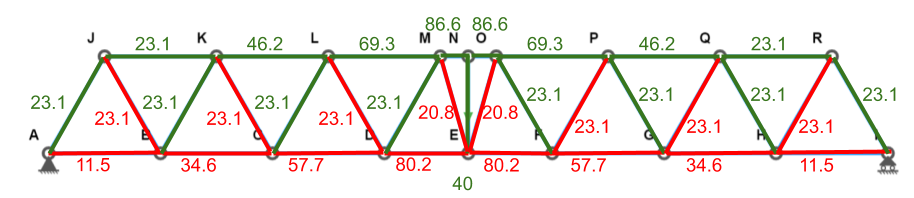
\includegraphics[scale=0.5]{ForceModel}
\end{center}

\section{Work Equalization Summary}
\large
\begin{center}
    \begin{tabular}{ |c|@{\hspace{20em}}| } 
        \hline
        Robert Li has worked on:\\
        \hline
        Joshua Liu has worked on:\\
        \hline
        Mitchell Green has worked on:\\
        \hline
    \end{tabular}
\end{center}
\normalsize
\bibliographystyle{apacite}
\nocite{*}
\bibliography{References}

%%% End document
\end{document}